%---------------------------------------------------
%----- Version History
%---------------------------------------------------
\subsubsection{Version History}\label{sec:version_history}
The version history $H$ is a set of documents. An update of an existing document in the Centrifuge protocol happens by creating a new version and linking this new version to the previously existing version. 
We define the set of all documents as $D$:
\begin{equation}
d \in D
\end{equation}
Every node keeps a history of all versions of a document in which they are listed as a collaborator.
\begin{equation}
H = (d_{[0]},...,d_{[n]})
\end{equation}
\newline
In the initial version of a document $d_0$, the current version and the identifier will be equal.
\begin{equation}
d_{[0]{\texttt{id}}} = d_{[0]\texttt{current}}
\end{equation}
\newline
The fields for the previous document root hash $D_{\texttt{prev-root}}$ and for the $D_{\texttt{prev}}$ id will be empty in the initial version.
\begin{eqnarray}
d_{[0]{\texttt{prev-root}}}& = & \emptyset \\
d_{[0]{\texttt{prev}}} & = & \emptyset
\end{eqnarray}
\newline
For all other documents $D$ in a version history $H$, the following conditions must be true:
\newline
\newline
Every document in a version history $H$ must have the same identifier.
\begin{equation}
\{d_{[i]} \in H \mid \forall d_{[j]} \in H :d_{[i]\texttt{id}} = d_{[j]\texttt{id}} \}
\end{equation}
\newline
The next version field of a document must be equal to the current version field of the successor document.
\begin{equation}
d_{[i]\texttt{next}} = d_{[i+1]\texttt{current}} 
\end{equation}
\newline
The previous version field of a document must be equal to the current version field of the predecessor document.
\begin{equation}
d_{[i]\texttt{prev}} = d_{[i-1]\texttt{current}} 
\end{equation}
\newline
The previous root hash of a document must be equal to the document root hash of the predecessor document.
\begin{equation}
d_{[i]\texttt{prev-root}} = d_{[i-1]\texttt{doc-root}}
\end{equation}
\newline
The history of the document can therefore be seen as a doubly linked list. Every document has the document hash $D_{\texttt{previous}}$ of the predecessor document and defines the $D_{\texttt{id}}$ of the next one. A node which performs a document update defines the the next version identifier $D_{\texttt{next}}$.
\begin{equation}
d_{[i]\texttt{next-img}} = \texttt{RAND32()}
\end{equation}
\begin{equation}
d_{[i]\texttt{next}} = \mathtt{sha256}(d_{[i]\texttt{next-img}})
\end{equation}
\newline
The field $D_{\texttt{next-img}}$ is needed for commit reveal scheme in the \textit{AnchorRepository} to prevent malicious anchoring of documents by non-collaborators. The function $\texttt{RAND32()}$ is a cryptographically secure random function and returns a byte 32 array. The function $\mathtt{sha256}$ denotes hash function SHA-2 256.
\\\\By referencing the previous root each state $d$, the history becomes an immutable attribute committed to in each version. To traverse the history $H$, one can follow the $d_{\mathtt{prev-root}}$ and $d_{\mathtt{prev}}$. To move forward in the list of history, $H$, one can go from $d_{\mathtt{next}}$ to $d_{\mathtt{current}}$.
\begin{figure}[thpb]
  \centering
  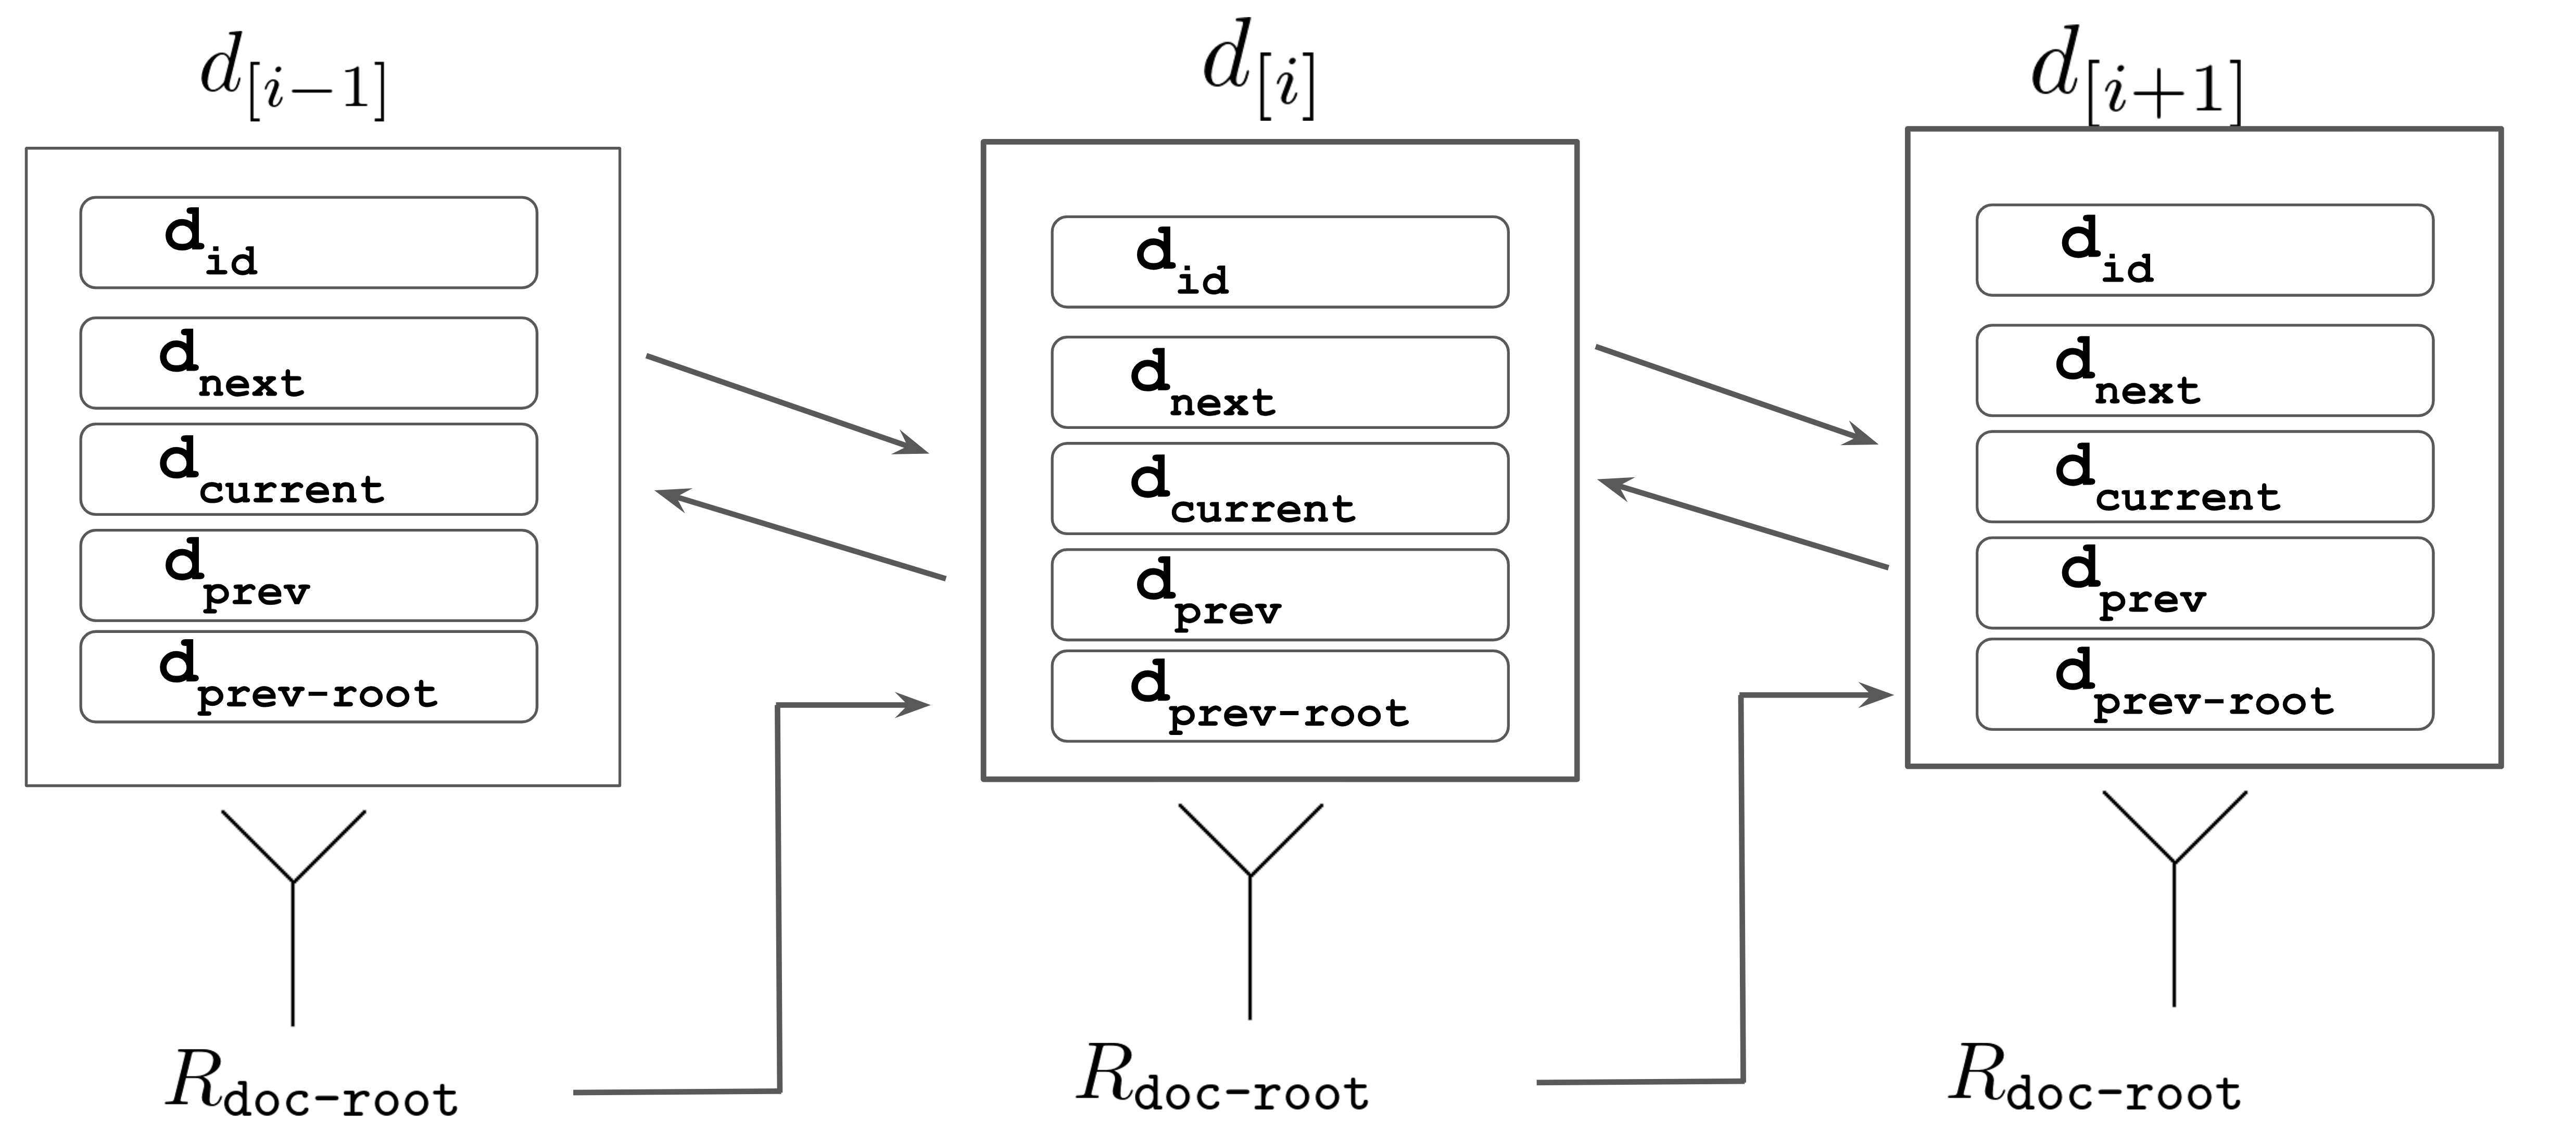
\includegraphics[width=16cm]{img/documents-history-v2.png}
  \caption{Doubly linked list of different versions of a document} 
  \label{fig:documents}
\end{figure}

